\hypertarget{cmsis__compiler_8h}{}\section{Dokumentacja pliku S\+T\+M/\+W\+D\+S\+\_\+\+Kosc\+\_\+\+Linux/\+Drivers/\+C\+M\+S\+I\+S/\+Include/cmsis\+\_\+compiler.h}
\label{cmsis__compiler_8h}\index{S\+T\+M/\+W\+D\+S\+\_\+\+Kosc\+\_\+\+Linux/\+Drivers/\+C\+M\+S\+I\+S/\+Include/cmsis\+\_\+compiler.\+h@{S\+T\+M/\+W\+D\+S\+\_\+\+Kosc\+\_\+\+Linux/\+Drivers/\+C\+M\+S\+I\+S/\+Include/cmsis\+\_\+compiler.\+h}}


C\+M\+S\+IS compiler generic header file.  


{\ttfamily \#include $<$stdint.\+h$>$}\newline
Wykres zależności załączania dla cmsis\+\_\+compiler.\+h\+:\nopagebreak
\begin{figure}[H]
\begin{center}
\leavevmode
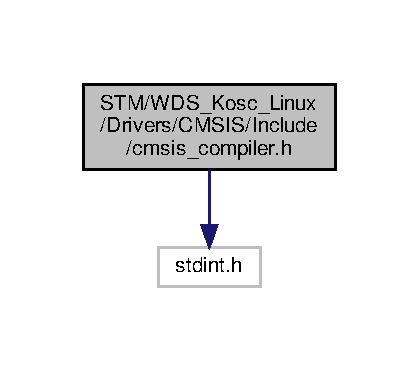
\includegraphics[width=201pt]{cmsis__compiler_8h__incl}
\end{center}
\end{figure}
Ten wykres pokazuje, które pliki bezpośrednio lub pośrednio załączają ten plik\+:\nopagebreak
\begin{figure}[H]
\begin{center}
\leavevmode
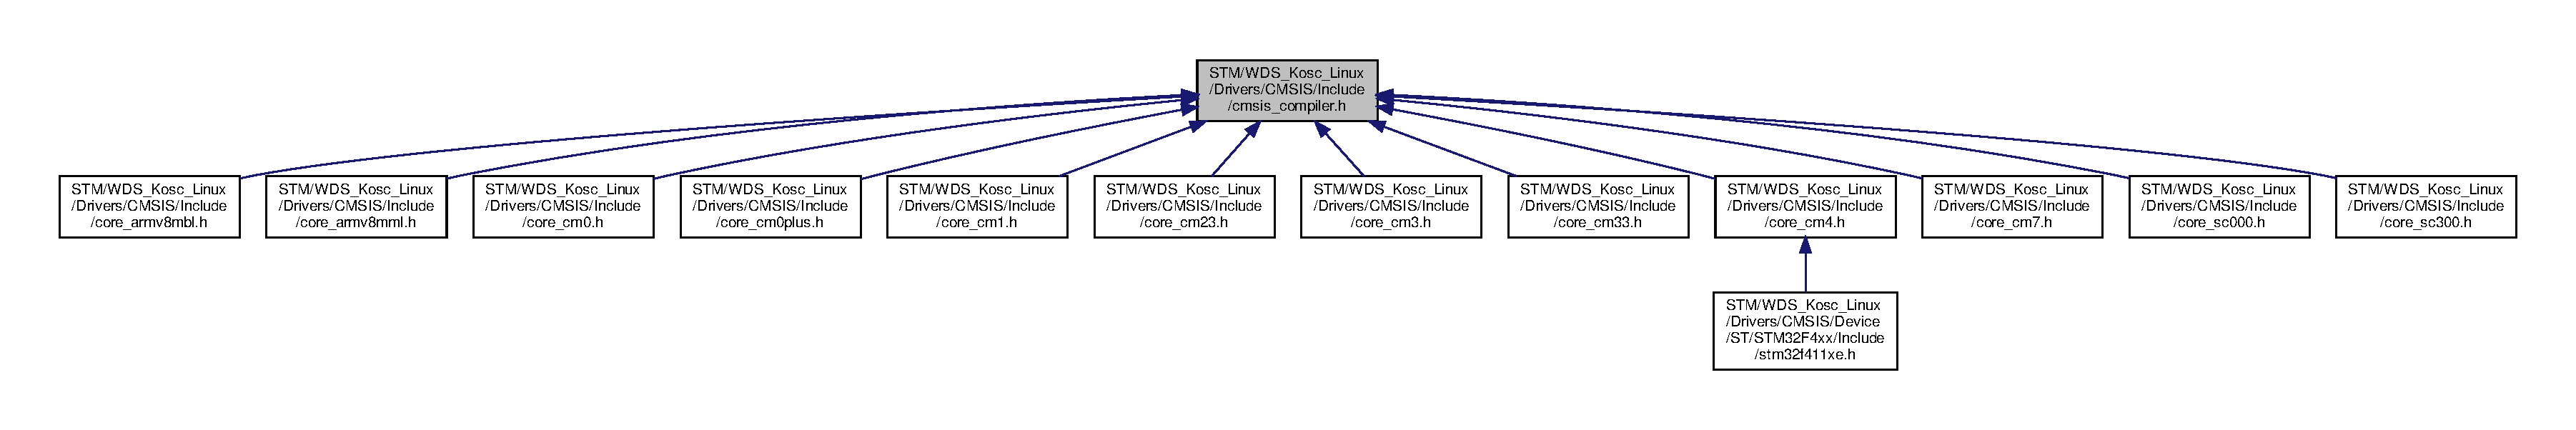
\includegraphics[width=350pt]{cmsis__compiler_8h__dep__incl}
\end{center}
\end{figure}


\subsection{Opis szczegółowy}
C\+M\+S\+IS compiler generic header file. 

\begin{DoxyVersion}{Wersja}
V5.\+0.\+4 
\end{DoxyVersion}
\begin{DoxyDate}{Data}
10. January 2018 
\end{DoxyDate}
